\documentclass[11pt]{article}
\usepackage[margin=1in]{geometry}
\usepackage{booktabs}
\usepackage{graphicx}
\usepackage{hyperref}
\usepackage{amsmath}
\usepackage{enumitem}
\usepackage[hyphens]{url}
\usepackage{listings}
\lstset{
  language=Python,
  basicstyle=\ttfamily\small,
  keywordstyle=\bfseries,
  frame=single,
  breaklines=true,
  columns=fullflexible,
  aboveskip=6pt,
  belowskip=6pt,
}
\setlength{\parindent}{0pt}
\setlength{\parskip}{6pt}

\title{\vspace{-1em}\textbf{Midway Check-in Report} \\ CS2650, Spring 2026\vspace{-0.5em}}
\author{Kayden Kehe}
\date{\vspace{-2em}}

\begin{document}
\maketitle

\section{Introduction}

For the midway check-in, we build a computation graph profiler for PyTorch that captures per-operator timing and memory statistics across a full training iteration (forward pass, backward pass, and optimizer step). The profiler instruments traced computational graphs, executing each node while recording wall-clock time and change in GPU memory usage. It classifies every tensor as a parameter, gradient, activation, or other allocation, and performs static analysis on activations to determine the number of graph nodes between an activation's last use in the forward pass and its first use in the backward pass (its \emph{idle gap}).

These profiling results establish the baseline measurements needed to guide the activation checkpointing algorithm in Phase~2. We profile two models (ResNet-152 and BERT) using batch sizes from 2 to 256 (ResNet) and 2 to 512 (BERT) on an NVIDIA A40 GPU.

\section{Problems Tackled}

\begin{itemize}[nosep]
\item \textbf{[Per-operator profiling]} Collecting fine-grained computation time and memory usage for every operator in the computational graph, executed in topological order.
\item \textbf{[Tensor classification]} Categorizing graph tensors as parameters, gradients, activations, or other allocations to understand the memory breakdown.
\item \textbf{[Activation idle-gap analysis]} Computing the static lifetime of each activation to identify candidates for checkpointing.
\item \textbf{[Memory scaling characterization]} Measuring how peak GPU memory and activation memory scale with batch size across two distinct models.
\end{itemize}

\section{Technical Description}

\subsection{Per-Operator Profiling}

\begin{enumerate}[label=\alph*),nosep,leftmargin=*]
\item \textbf{Problem framing.}
To decide which activations to checkpoint, we first need to know the computational cost and memory footprint of every operation in the training graph. PyTorch's built-in profiler provides aggregate statistics but does not expose per-node memory deltas in the context of the full forward--backward--optimizer graph. We need a profiler that walks the graph in topological order and records, for each node, its execution time and the change in GPU memory it causes.

\item \textbf{High-level solution.}
We extend the provided graph interpreter to instrument each node execution. Before and after executing a node, we query the current GPU memory allocation and take the difference. We also bracket each call with GPU event pairs to measure wall-clock time. Multiple runs (5 warmup + 5 measured) are executed and averaged to reduce noise. Peak GPU memory is tracked per-run and averaged across measured runs.

\item \textbf{Deeper details.}
We maintain a running cumulative sum of deltas that resets at the start of each run, record the per-run maximum, and average across measured runs. We also record the true GPU peak via \lstinline|torch.cuda.max_memory_allocated()|, since the cumulative-delta peak can overcount due to CUDA allocator memory reuse.\\

Parameters are already allocated before the graph executes (they appear as \texttt{placeholder} nodes with zero delta), and gradients are often allocated in-place during backward kernels. Neither contributes a visible positive delta at its own node, so most backward-pass memory is classified as OTHER, under-attributing memory to the PARAM and GRAD categories. The activation category is reliable, though, since each activation node produces a fresh output tensor whose allocation is captured by the delta.
\end{enumerate}

\subsection{Tensor Classification and Memory Breakdown}

\begin{enumerate}[label=\alph*),nosep,leftmargin=*]
\item \textbf{Problem framing.}
A raw list of memory deltas per node is not actionable. To understand \emph{where} memory goes during training, we need to classify each tensor into one of four categories: parameters, gradients, activations, and other (optimizer state, temporary buffers, etc.).

\item \textbf{High-level solution.}
Parameter and gradient nodes are easily located by observing the arguments in the \texttt{\_fused\_adam} node. Activation nodes are forward-pass outputs consumed by at least one backward-pass node. Everything else is classified as OTHER. To identify whether a node exists on the forward or backward pass, we insert a dummy separator node to flag the position in the graph.

\item \textbf{Deeper details.}
There really aren't deeper details here!

\begin{table}[h]
\centering
\caption{Computational graph overview.}
\label{tab:overview}
\begin{tabular}{lrr}
\toprule
 & \textbf{ResNet-152} & \textbf{BERT} \\
\midrule
Total graph nodes   & 8{,}681 & 4{,}352 \\
Parameters          & 467     & 201     \\
Activations         & 778     & 324     \\
Gradients           & 467     & 201     \\
Other               & 6{,}969 & 3{,}626 \\
Unique op types     & 30      & 36      \\
\bottomrule
\end{tabular}
\end{table}
\end{enumerate}

\subsection{Activation Idle-Gap Analysis}

\begin{enumerate}[label=\alph*),nosep,leftmargin=*]
\item \textbf{Problem framing.}
Activation checkpointing discards activations that occupy memory for a long time, recomputing them when needed in the backward pass. To identify the best candidates, we need to quantify how long each activation sits idle, measured as the number of intervening graph nodes between its last forward use and its first backward use.

\item \textbf{High-level solution.}
For each activation, we perform a static analysis over the graph's dependency edges, recording the topological index of its last forward consumer and first backward consumer. We rank activations for checkpointing consideration by computing $\text{size} \times \text{idle\_gap}$.

\item \textbf{Deeper details.}
Table~\ref{tab:ac_candidates} shows the top checkpointing candidates at batch size 32.

\begin{table}[h]
\centering
\caption{Top 5 AC candidates by memory-time score (BS=32).}
\label{tab:ac_candidates}
\begin{tabular}{llrrr}
\toprule
\textbf{Model} & \textbf{Activation} & \textbf{Size (MB)} & \textbf{Idle Gap} & \textbf{Score} \\
\midrule
ResNet-152 & convolution   & 98.0 & 2{,}595 & 254{,}310 \\
           & convolution\_3 & 98.0 & 2{,}542 & 249{,}116 \\
           & convolution\_4 & 98.0 & 2{,}528 & 247{,}744 \\
           & convolution\_7 & 98.0 & 2{,}478 & 242{,}844 \\
           & convolution\_10 & 98.0 & 2{,}428 & 237{,}944 \\
\midrule
BERT       & add\_1  & 12.0 & 1{,}901 & 22{,}812 \\
           & add\_2  & 12.0 & 1{,}797 & 21{,}564 \\
           & add\_3  & 12.0 & 1{,}746 & 20{,}952 \\
           & add\_4  & 12.0 & 1{,}642 & 19{,}704 \\
           & add\_5  & 12.0 & 1{,}591 & 19{,}092 \\
\bottomrule
\end{tabular}
\end{table}

For ResNet-152, the top candidates are early convolution layers producing large feature maps (98~MB each) with idle gaps exceeding 2{,}400 nodes. For BERT, the candidates are residual addition outputs at layer-norm boundaries---each 12~MB with idle gaps of 1{,}000--1{,}900 nodes. ResNet-152 has a median idle gap of 0 but a mean of 515, indicating a long tail. BERT has a median of 596 and mean of 700.\\

Figure~\ref{fig:waterfall} shows cumulative memory over the course of graph execution. The forward pass (left of the dashed separator) builds up activation memory steadily, while the backward pass continues to increase cumulative memory due to gradient and optimizer state allocations. For ResNet-152, the forward-pass memory ramp is steep---large convolution feature maps accumulate quickly. For BERT, the ramp is more gradual, consistent with its smaller per-activation sizes.

\begin{figure}[h]
\centering
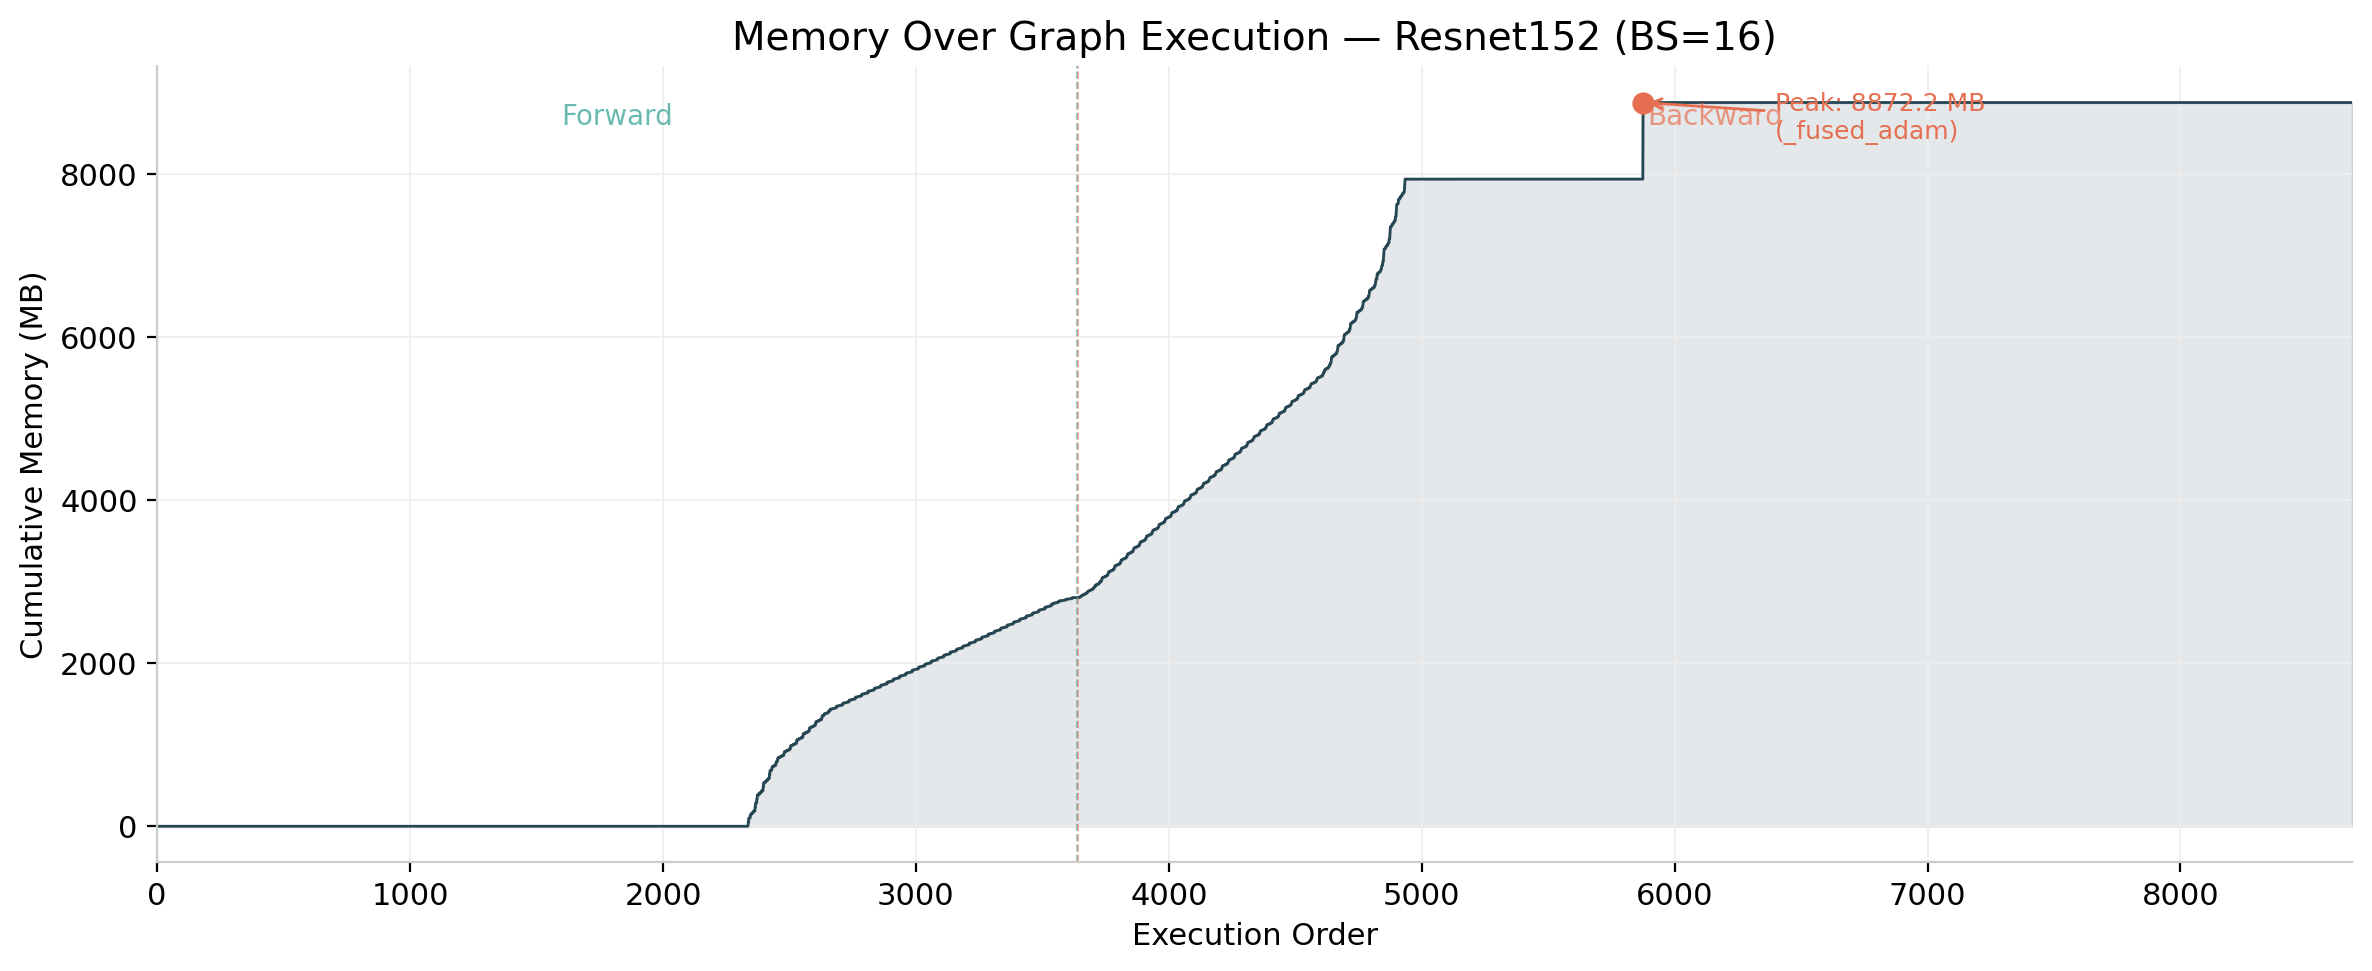
\includegraphics[width=0.8\textwidth]{plots/resnet152/waterfall.png}
\\
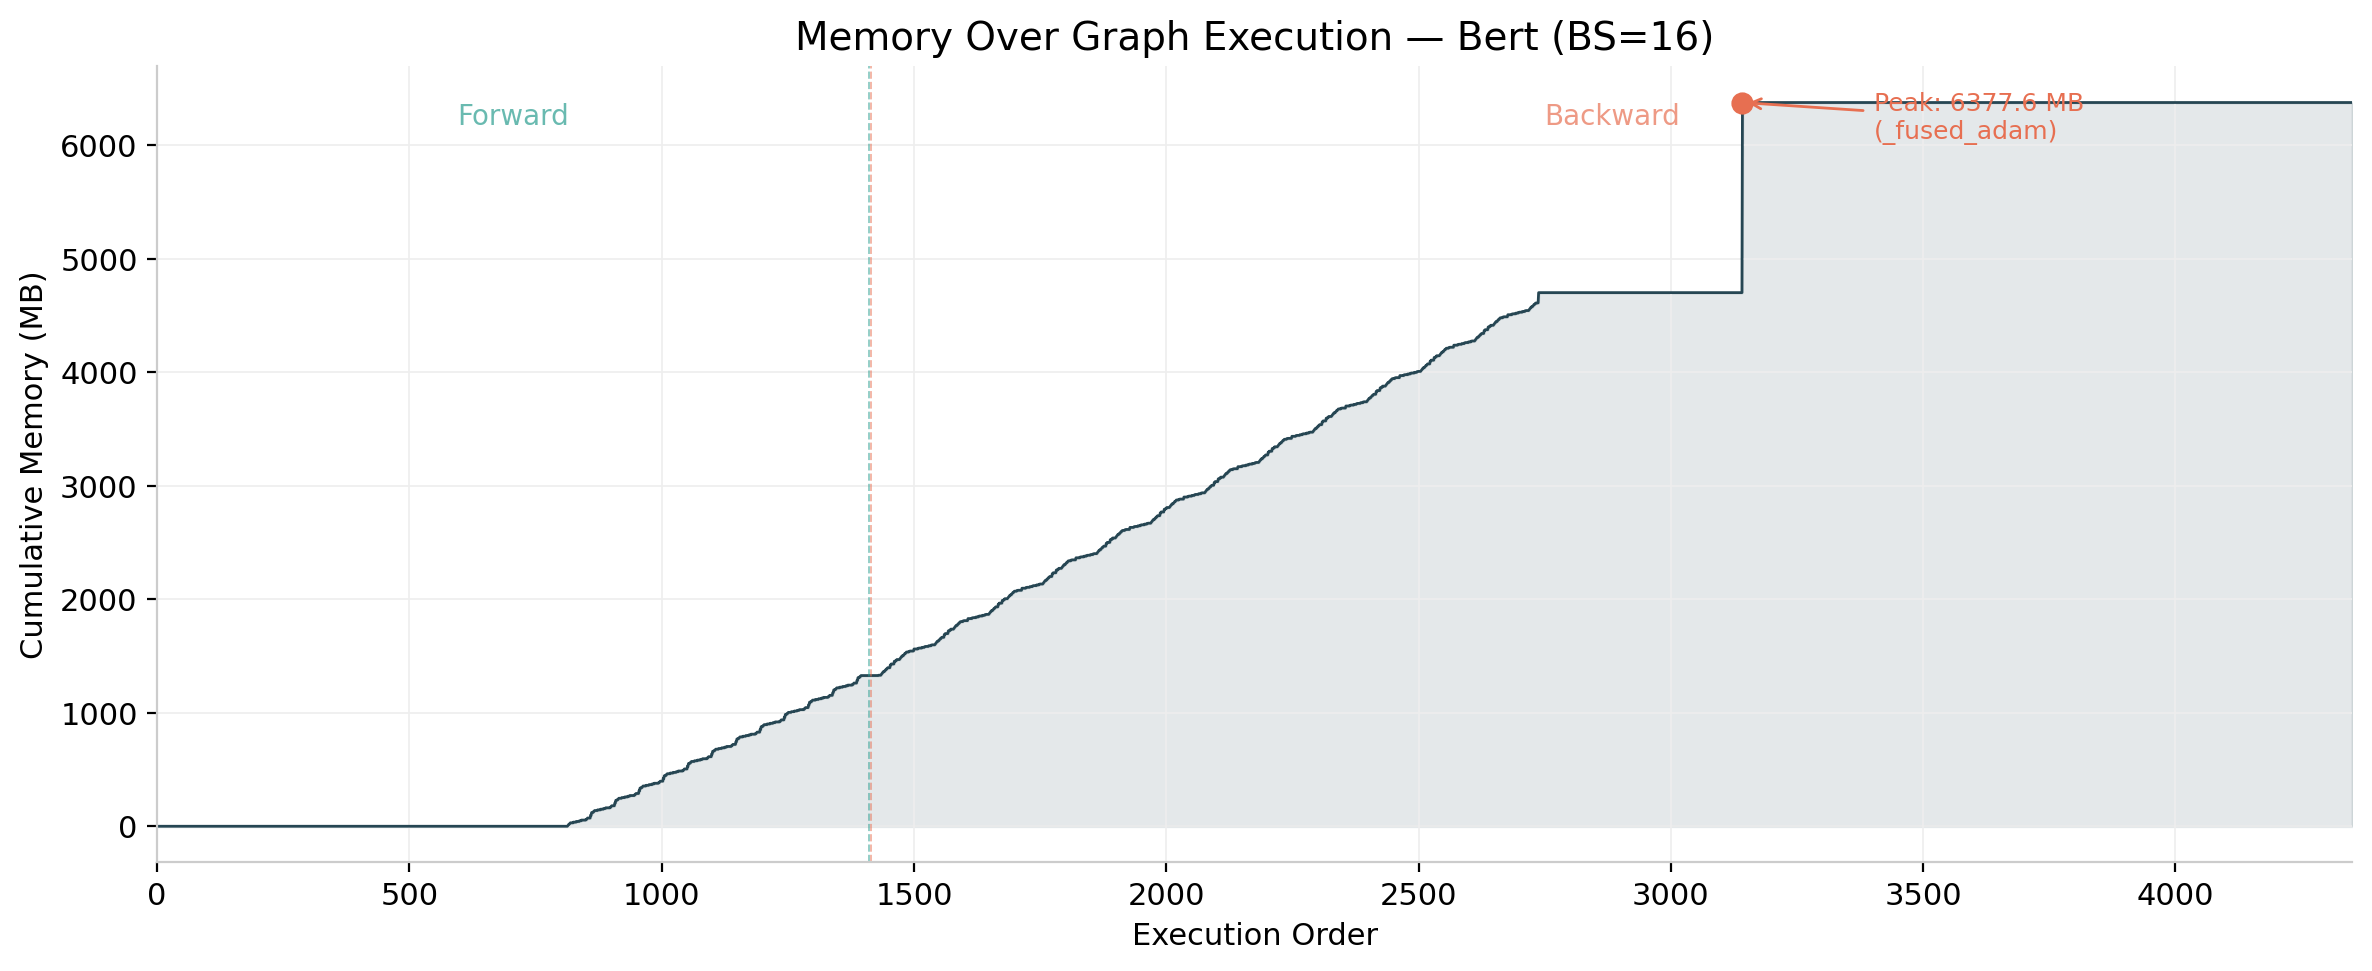
\includegraphics[width=0.8\textwidth]{plots/bert/waterfall.png}
\caption{Cumulative memory over graph execution for ResNet-152 (left) and BERT (right) at BS=16. The dashed line marks the forward--backward boundary.}
\label{fig:waterfall}
\end{figure}

If all activations were checkpointed, the theoretical maximum memory reduction would be 44.8\% of peak GPU memory for ResNet-152 and 8.2\% for BERT (at BS=32). ResNet-152's activations (2{,}767~MB) dominate its 6{,}177~MB peak, while BERT's activations (300~MB) are small relative to its 3{,}645~MB of parameters and optimizer state.
\end{enumerate}

\subsection{Memory and Timing Scaling}

\begin{enumerate}[label=\alph*),nosep,leftmargin=*]
\item \textbf{Problem framing.}
Understanding how memory and compute scale with batch size is essential for predicting when activation checkpointing will be most beneficial. We need to characterize this scaling behavior empirically.

\item \textbf{High-level solution.}
We sweep batch sizes across both models, recording peak GPU memory, activation memory, and forward/backward time at each point. We compute per-sample memory and memory doubling factors to assess linearity.

\item \textbf{Deeper details.}
Table~\ref{tab:scaling} shows selected scaling results.

\begin{table}[h]
\centering
\caption{Memory and timing scaling across batch sizes.}
\label{tab:scaling}
\begin{tabular}{lrrrrrr}
\toprule
& \multicolumn{3}{c}{\textbf{ResNet-152}} & \multicolumn{3}{c}{\textbf{BERT}} \\
\cmidrule(lr){2-4} \cmidrule(lr){5-7}
\textbf{BS} & \textbf{GPU (MB)} & \textbf{Act (MB)} & \textbf{Time (ms)} & \textbf{GPU (MB)} & \textbf{Act (MB)} & \textbf{Time (ms)} \\
\midrule
2   & 1{,}884  & 176     & 274   & 3{,}362  & 19    & 179   \\
8   & 2{,}126  & 695     & 292   & 3{,}382  & 75    & 192   \\
32  & 6{,}177  & 2{,}767 & 421   & 3{,}645  & 300   & 306   \\
128 & 22{,}496 & 11{,}028 & 929  & 10{,}746 & 1{,}200 & 689 \\
256 & 44{,}278 & 22{,}055 & 1{,}993 & 20{,}220 & 2{,}401 & 1{,}217 \\
\bottomrule
\end{tabular}
\end{table}

Figure~\ref{fig:mem_vs_batch} shows peak GPU memory as a function of batch size.

\begin{figure}[h]
\centering
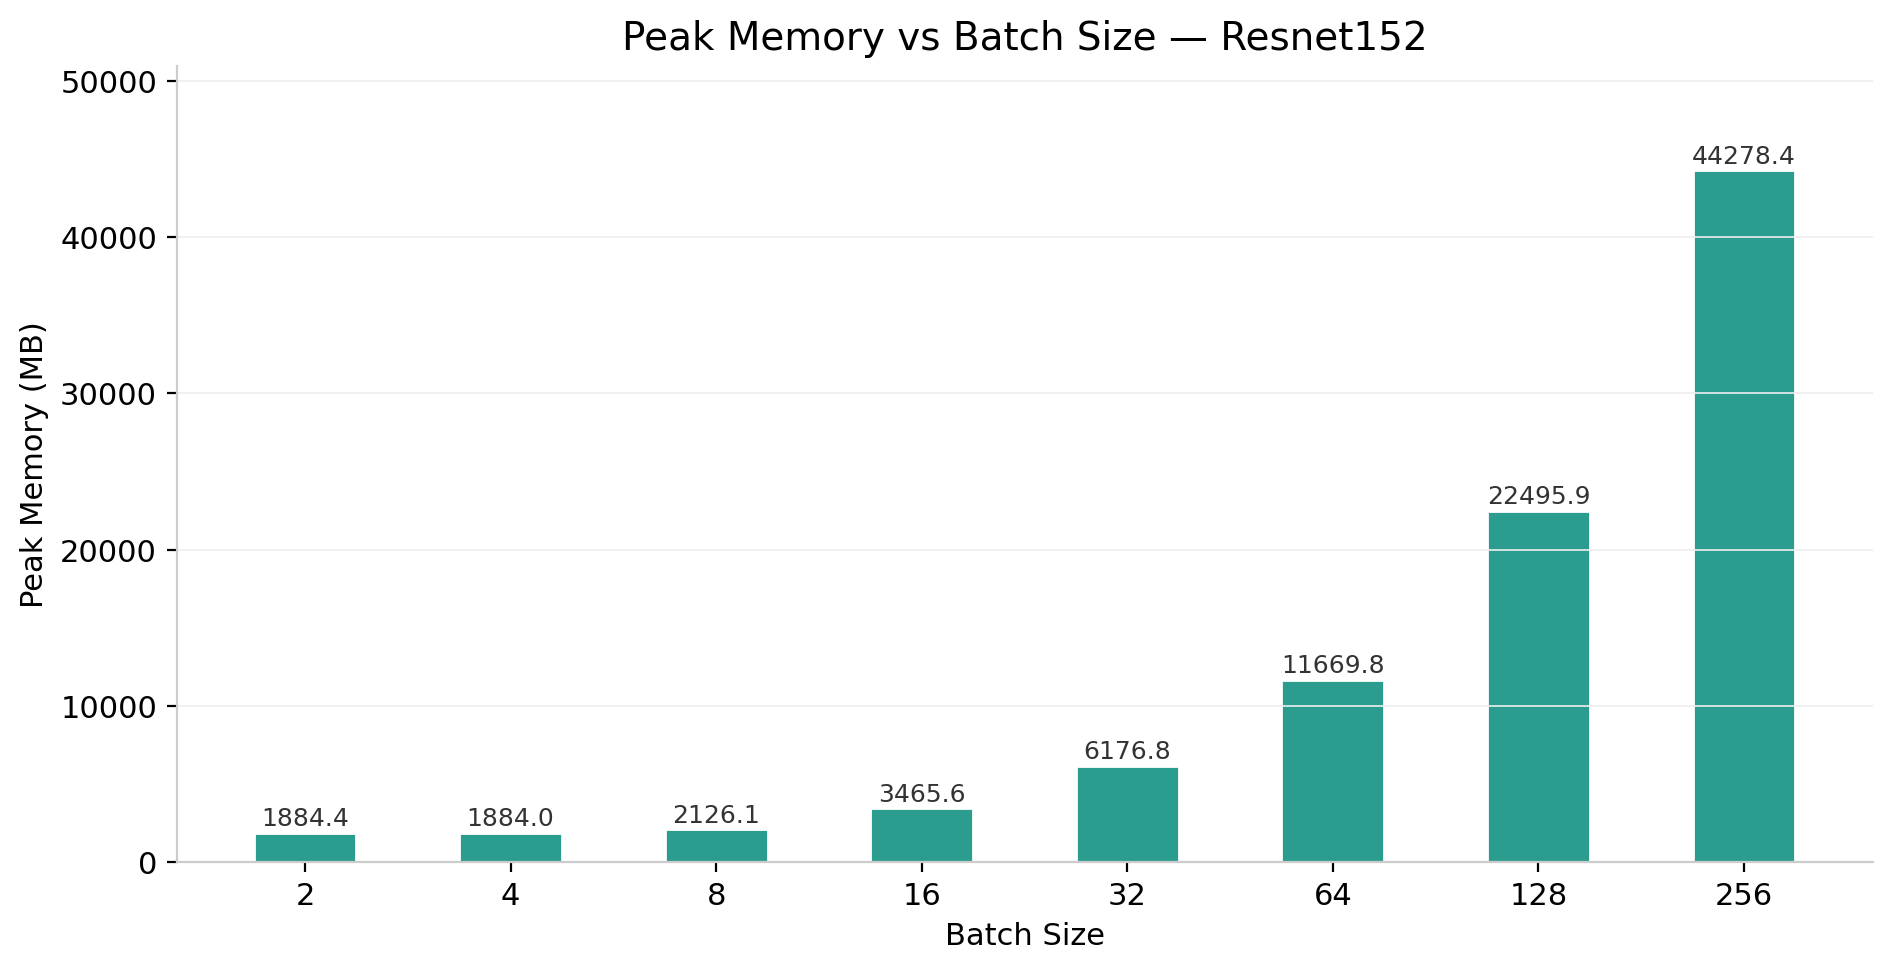
\includegraphics[width=0.48\textwidth]{plots/resnet152_memory_vs_batch.png}
\hfill
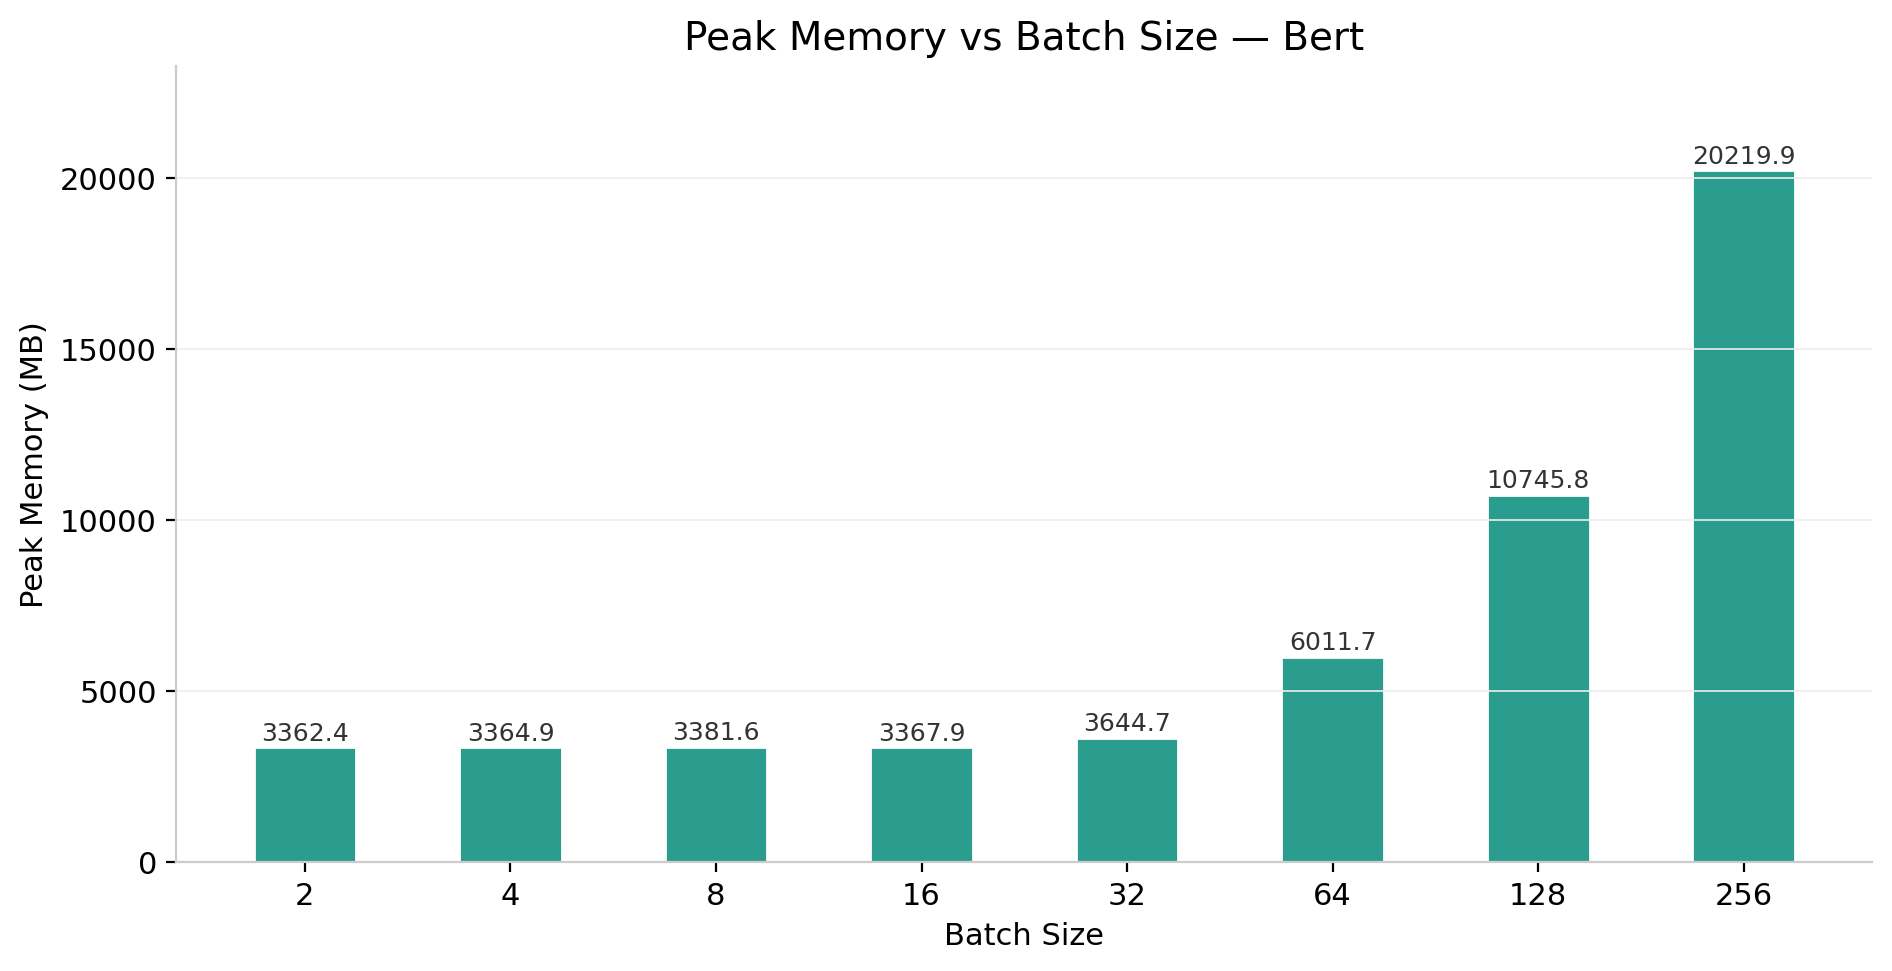
\includegraphics[width=0.48\textwidth]{plots/bert_memory_vs_batch.png}
\caption{Peak GPU memory vs.\ batch size for ResNet-152 (left) and BERT (right).}
\label{fig:mem_vs_batch}
\end{figure}

Key observations:
\begin{itemize}[nosep]
\item Per-sample activation memory is nearly constant: ${\sim}$86.5~MB for ResNet-152 and ${\sim}$9.4~MB for BERT.
\item At small batch sizes, fixed costs (parameters, optimizer state) dominate space. At BS=128$\to$256, the factor is 1.97 for ResNet-152 and 1.88 for BERT.
\item Convolution and batch-norm (forward + backward) account for ${>}$40\% of ResNet-152 compute. Matrix multiplications account for ${\sim}$39\% of BERT compute.
\end{itemize}

Figure~\ref{fig:latency_vs_batch} shows iteration latency as a function of batch size.

\begin{figure}[h]
\centering
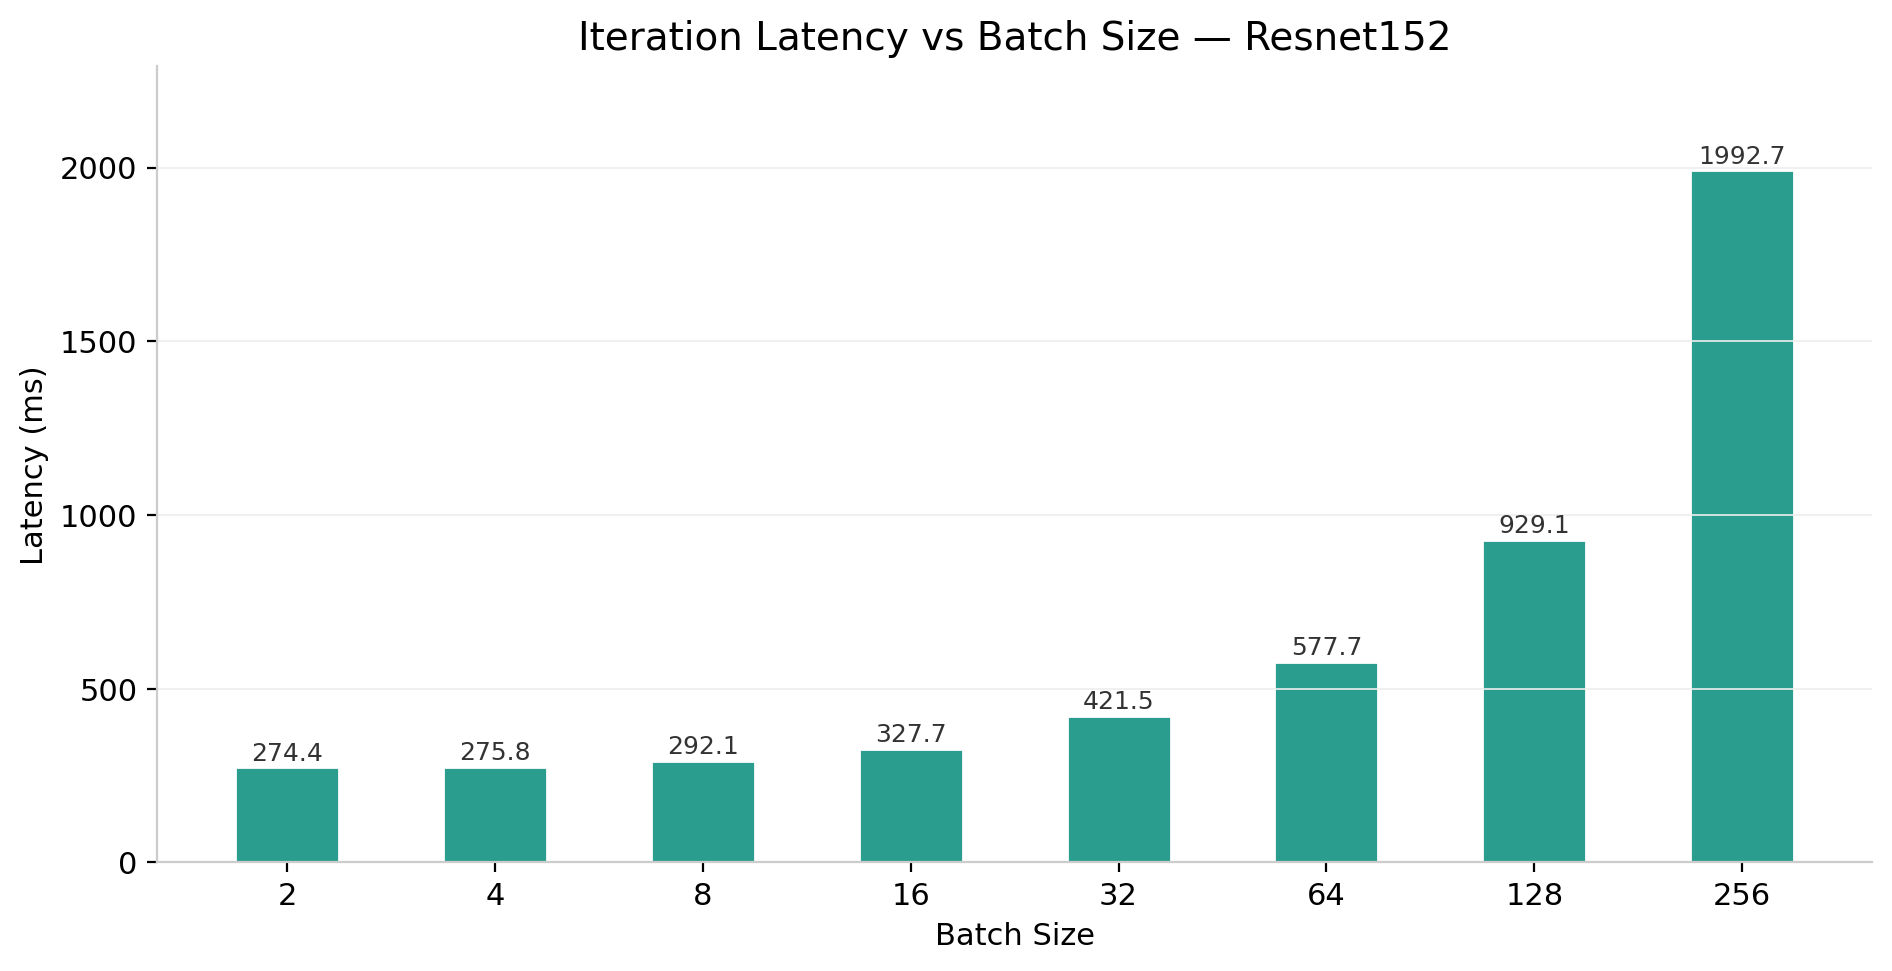
\includegraphics[width=0.48\textwidth]{plots/resnet152_latency_vs_batch.png}
\hfill
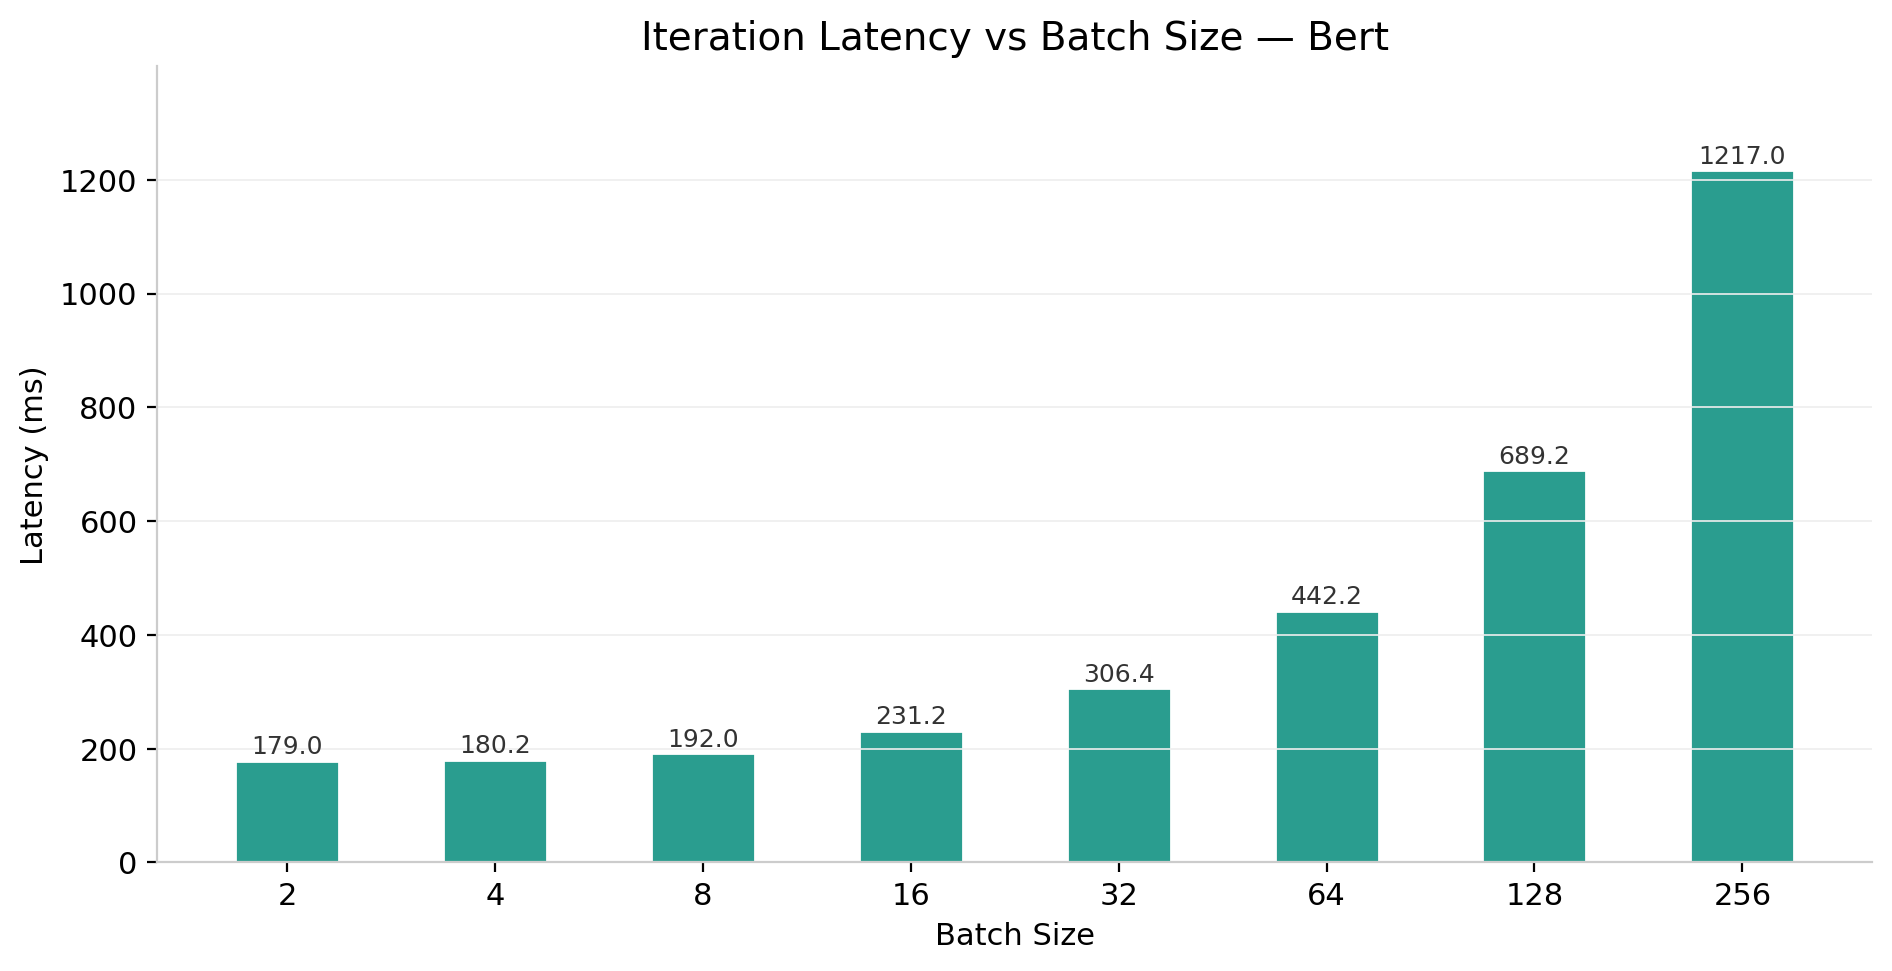
\includegraphics[width=0.48\textwidth]{plots/bert_latency_vs_batch.png}
\caption{Iteration latency vs.\ batch size for ResNet-152 (left) and BERT (right).}
\label{fig:latency_vs_batch}
\end{figure}

\end{enumerate}

\end{document}


